\documentclass[10pt,a4paper]{article}
\usepackage[utf8]{inputenc}
\usepackage{amsmath}
\usepackage{gensymb}
\usepackage{amsfonts}
\usepackage{siunitx}
\usepackage[european]{circuitikz}
\usepackage{geometry}
\newgeometry{tmargin=2cm, bmargin=2cm, lmargin=2cm, rmargin=2cm}
\usepackage{amssymb}
\usepackage{polski}
\usepackage{graphicx}
\author{\textbf{T. Fąs}}
\title{\textbf{ZAWARTOŚĆ IZOTOPU $^{40}$K W POTASIE NATURALNYM}}
\begin{document}
\maketitle

\begin{center}
\textbf{\subsection*{STRESZCZENIE}}
\end{center}
W doświadczeniu wyznaczono zawartość procentową $p$ radioizotopu $^{40}$K w solach potasu K$_{2}$CO$_{3}$. Otrzymano wartość $p=(0,0203\pm0,0012) \%$. Wartość ta jest prawie dwukrotnie wyższa od oczekiwanej, prawdopodobnie na skutek błędnie działającej aparatury. Oprócz tego wyznaczono energetyczną zdolność rozdzielczą spektrometru, która wynosi $(9,024\pm0,047)\%$.    


\begin{center}
\textbf{\subsection*{WSTĘP}}
\end{center}
W środowisku naturalnym występują trzy izotopy potasu: $^{39}$K, $^{40}$K i $^{41}$K, z czego tylko $^{40}$K jest radioaktywny. W 89$\%$ przypadków ulega on rozpadowi $\beta^{-}$. W pozostałych 11$\%$ przypadków dochodzi do emisji kwantu $\gamma$. W doświadczeniu mierzono liczbę rozpadów $\gamma$ w czasie 30 minut i na tej podstawie wyznaczono stosunek masy $^{40}$K do całości naturalnie występującego potasu. 

Jeśli w czasie $t$ odnotowano $N$ rozpadów, to z prawa zaniku promieniotwórczego można wyznaczyć początkową liczbę $N_{0}$ jąder $^{40}$K. Relacją między $N$ i $N_{0}$ dana jest następującym wzorem:
\begin{equation}
N=N_{0}\left(1-e^{-\lambda t} \right),
\end{equation}
gdzie $\lambda$ jest stałą rozpadu. Znając czas połowicznego zaniku $T_{1/2}=1,26\cdot10^9$ lat można go powiązać z wartością $\lambda$ następującą relacją:
\begin{equation}
\lambda=\dfrac{\ln 2}{T_{1/2}}.
\end{equation}

Znając masy molowe $^{39}$K i $^{40}$K oznaczone kolejno $m_{39}$ i $m_{40}$, całkowitą masę $M$ próbki soli K$_{2}$CO$_{3}$ oraz jej masę molową $m_{s}$ można wyznaczyć:

masę potasu $^{40}$K ze wzoru:
\begin{equation}
M_{40}=\dfrac{N_{0}}{N_{A}}m_{40},
\end{equation}
gdzie $N_{A}$ jest liczą Avogadra; masę $^{39}$K ze wzoru:
\begin{equation}
M_{39}=\left(\dfrac{2M}{m_{s}}-\dfrac{N_{0}}{N_{A}}\right)m_{39}
\end{equation}
oraz szukany stosunek $p=M_{40}/(M_{39}+M_{40})$.
\begin{center}
\textbf{\subsection*{UKŁAD DOŚWIADCZALNY}}
\end{center}
Układ doświadczalny składał się ze spektrometru podłączonego do komputera, próbki cezu $^{137}$Cs, kobaltu $^{60}$Co oraz próbki soli K$_{2}$CO$_{3}$ o masie $M=1011,91$g. Wykonano 15-minutowy pomiar widma cezu oraz pomiar widma kobaltu, węglanu potasu i tła, z czego każdy z tych pomiarów trwał po 30 minut. Wyniki zostały zapisane w pamięci komputera.

\begin{center}
\textbf{\subsection*{WYNIKI POMIARÓW}}
\end{center}
Wyniki pomiarów w postaci wykresów widm przedstawione są na Rysunkach 1-4.

\begin{figure}[h!]
\centering
\begin{minipage}{0.5\textwidth}
  \centering
  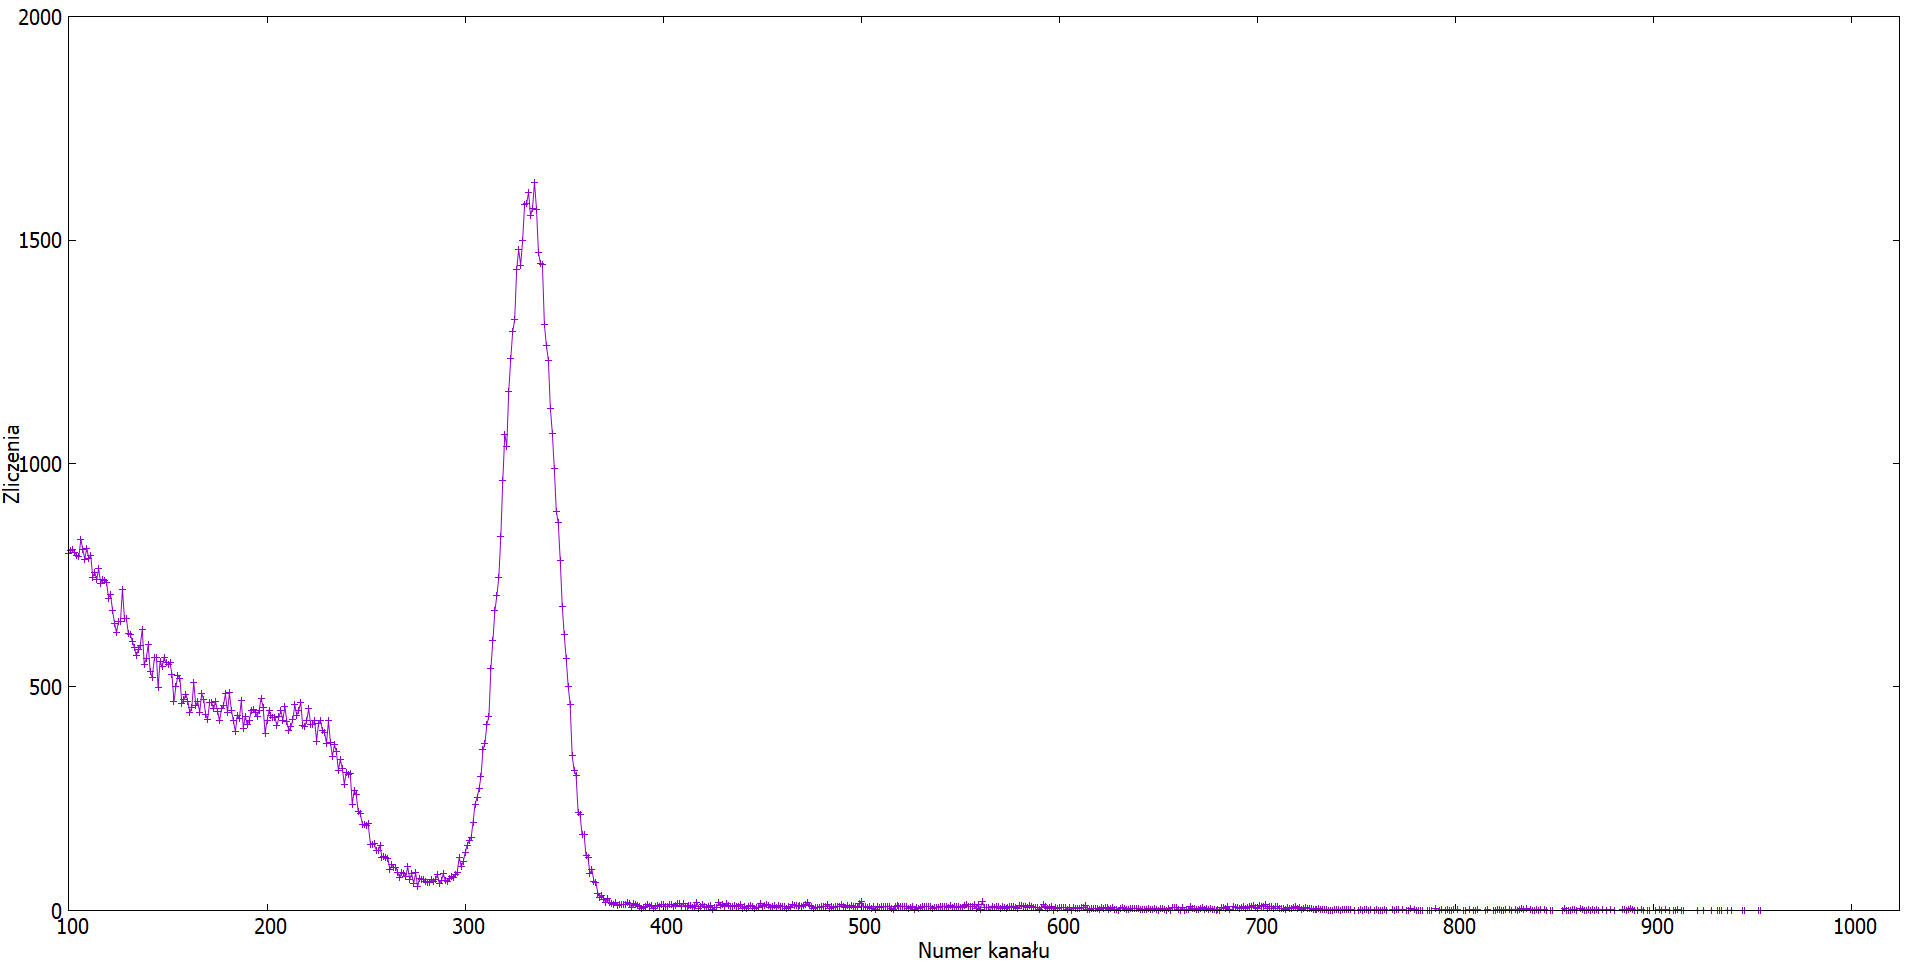
\includegraphics[width=8cm, height=5cm ]{rap14rys1} 
\caption{Widmo cezu.}
\end{minipage}%
\begin{minipage}{0.5\textwidth}
  \centering
  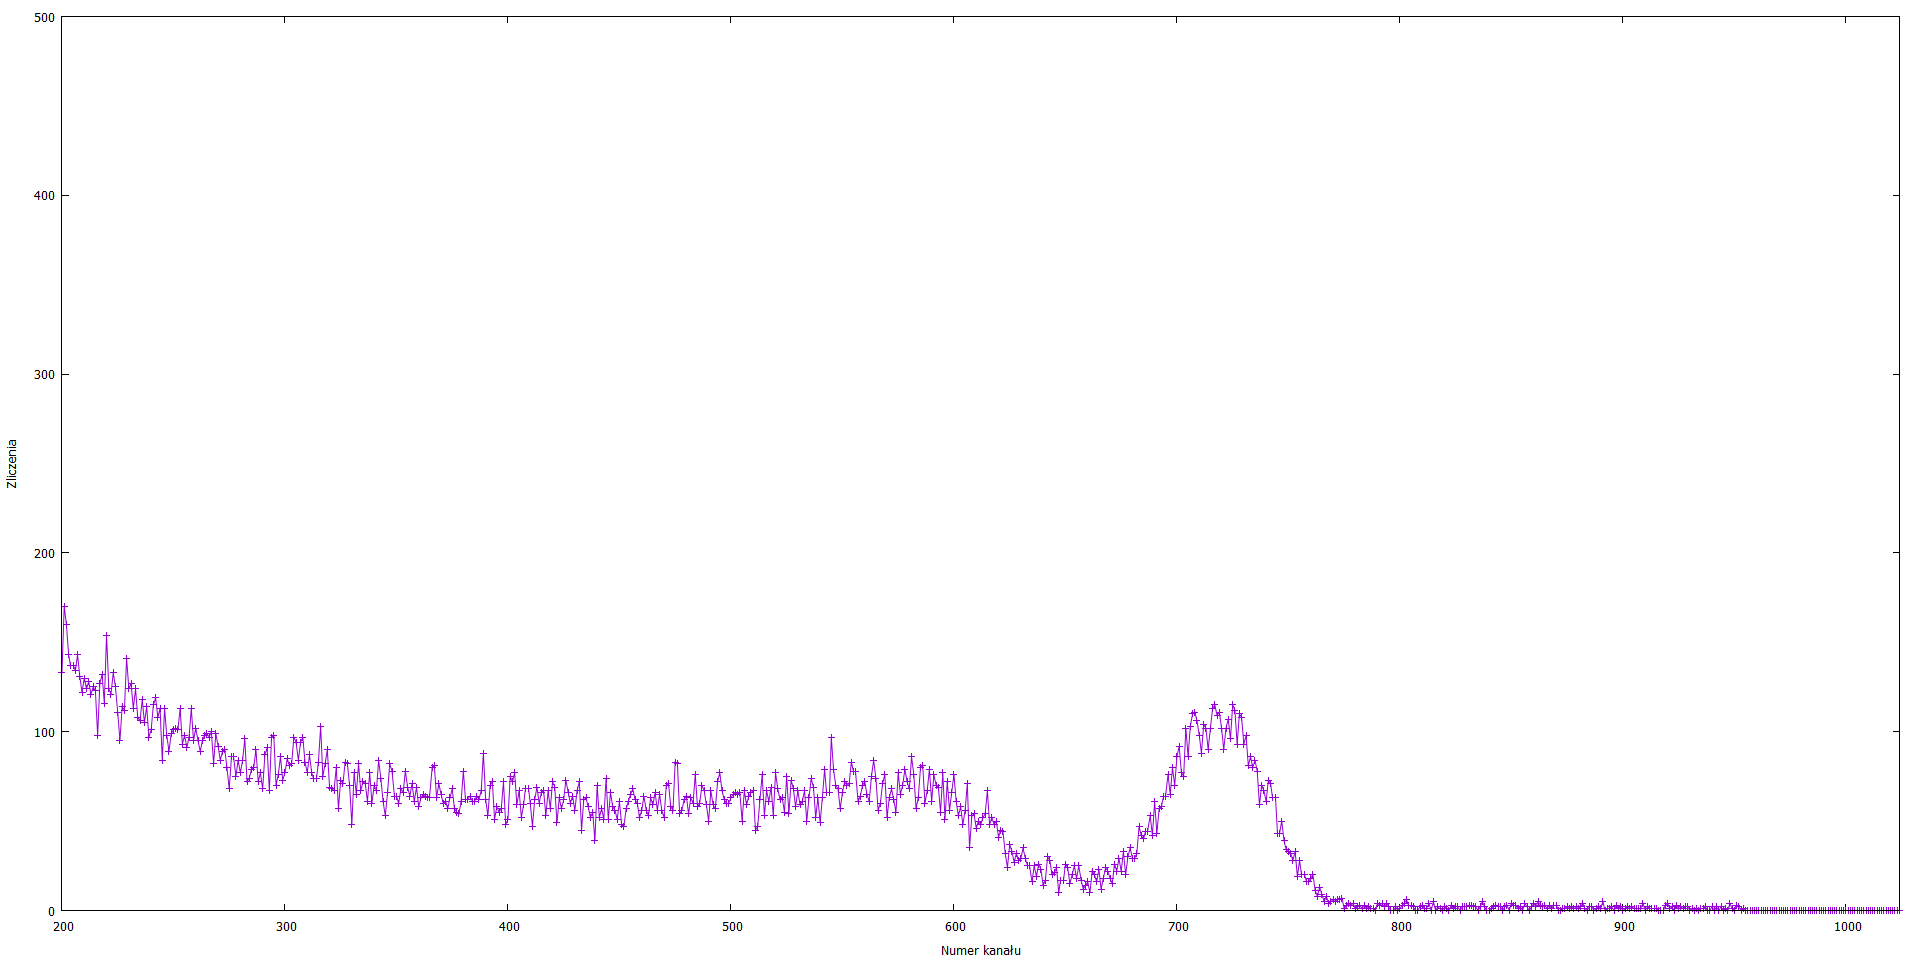
\includegraphics[width=8cm, height=5cm ]{rap14rys2} 
\caption{Widmo kobaltu.}
\end{minipage}
\end{figure}
\begin{figure}[h!]
\centering
\begin{minipage}{0.5\textwidth}
  \centering
  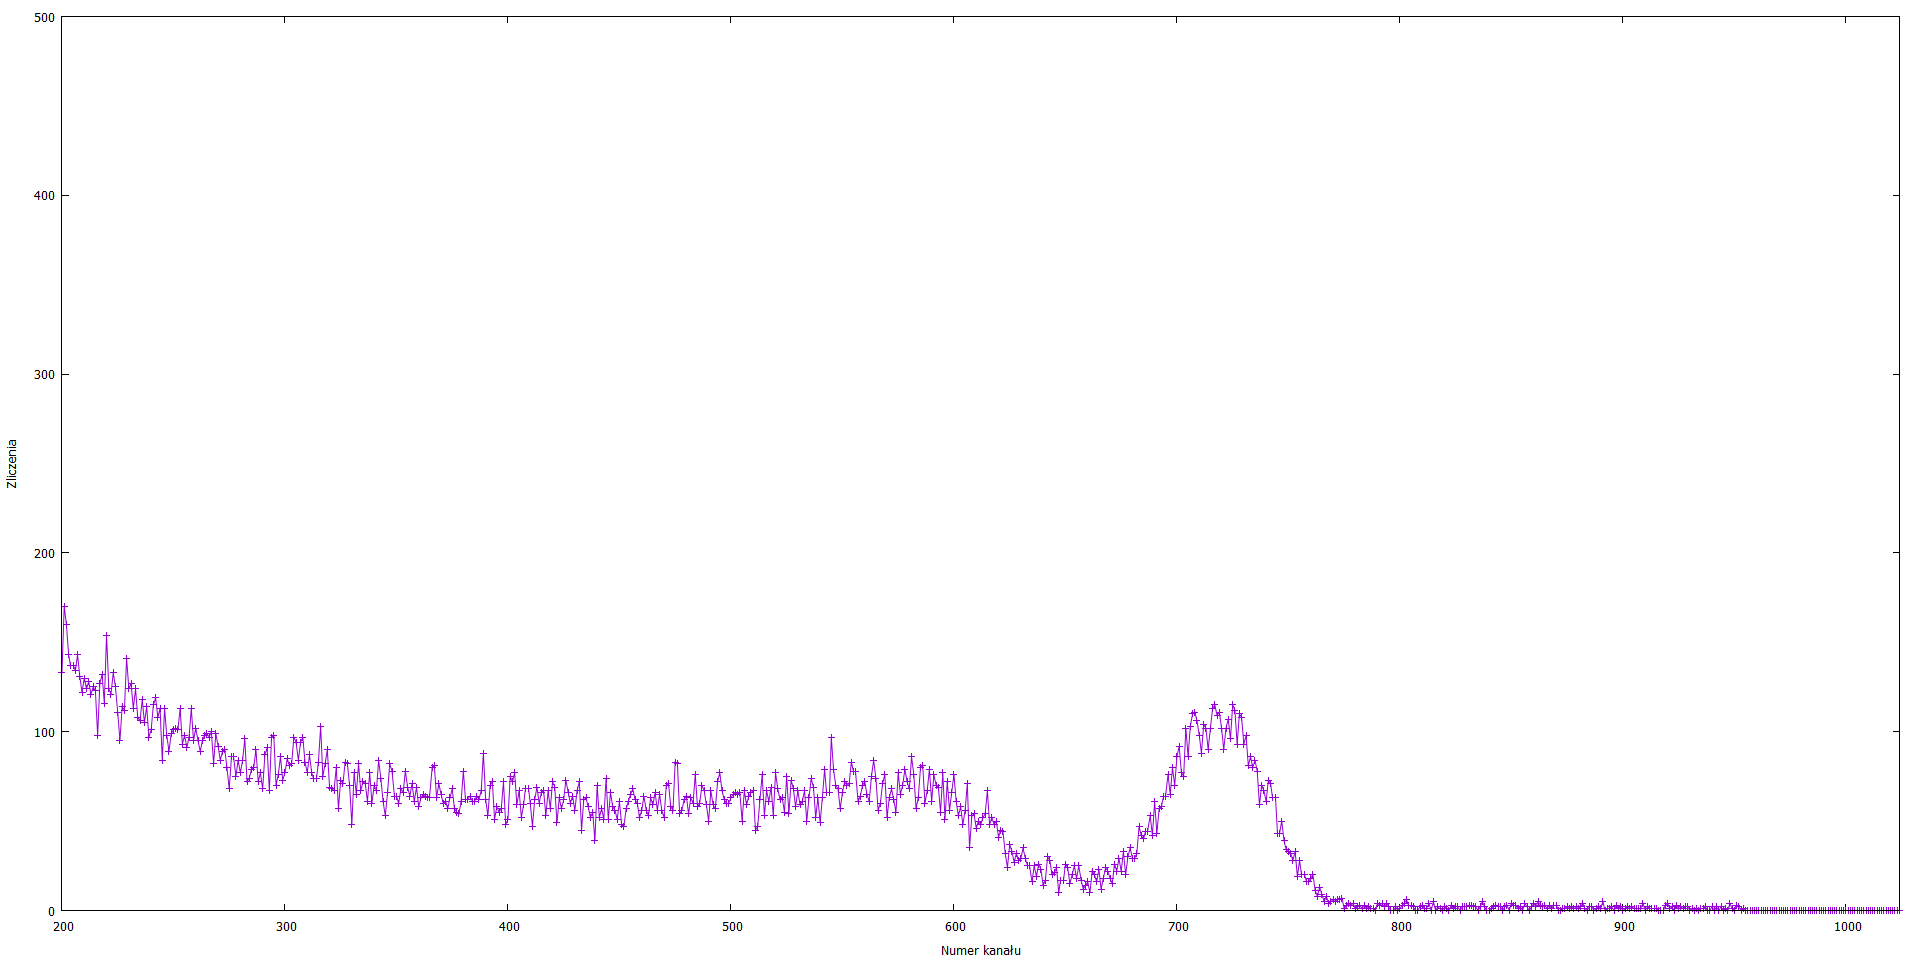
\includegraphics[width=8cm, height=5cm ]{rap14rys31} 
\caption{Widmo potasu.}
\end{minipage}%
\begin{minipage}{0.5\textwidth}
  \centering
  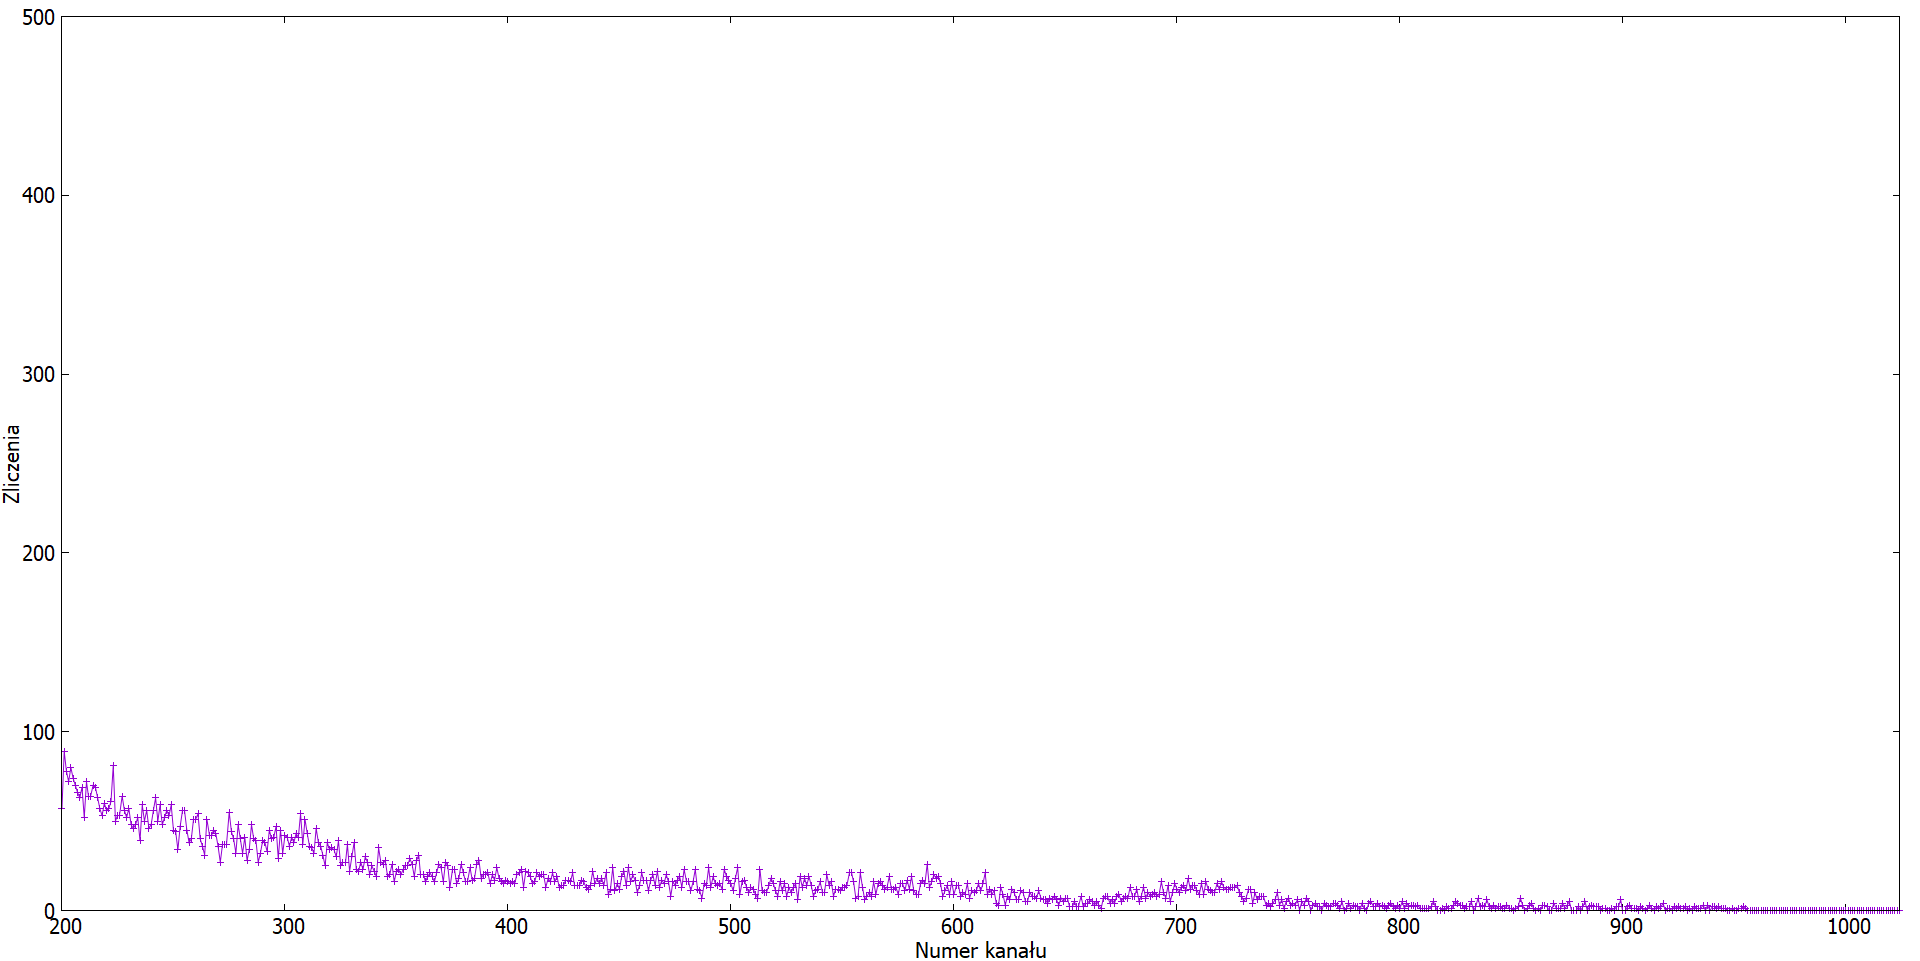
\includegraphics[width=8cm, height=5cm ]{rap14rys32} 
\caption{Widmo tła.}
\end{minipage}
\end{figure}


\begin{center}
\textbf{\subsection*{ANALIZA DANYCH}}
\end{center}

\begin{center}
\textbf{\subsection*{DYSKUSJA WYNIKÓW I WNIOSKI}}
\end{center} 

\begin{center}
\begin{thebibliography}{9}

 
\bibitem{tay1}
 J. R. Taylor,
 \emph{Wstęp do analizy błędu pomiarowego},
 PWN, Warszawa, 1995, s. 175.
 
 

 \end{thebibliography}

\end{center}


\end{document}